\titre{Principe :} A partir d'un sommet, on calcule un arbre couvrant sur les sommets accessibles à partir de ce sommet. \\
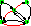
\includegraphics[width=200px]{Images/fig9.pdf}\\

\titre{Parcours en largeur :} On regarde les voisins du sommet, puis leurs voisins et ainsi de suite. Cela produit des chemins de longueur minimales du sommet de départ à tous les autres. \\

\titre{Exemple :} \\
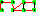
\includegraphics[width=200px]{Images/fig10.pdf}\\
\begin{tabular}{l|l|l|l|l|l|l|l|l}
 vu & V & V & V & V & V & V & V & V
\end{tabular} \\

\begin{tabular}{l|l|l|l|l|l|l|l|l}
 pere & 2 & - & 6 & 3 & 1 & 2 & 6 & 7
\end{tabular} \\

\begin{tabular}{l|l|l|l|l|l|l|l|l}
 dist & 1 & 0 & 2 & 3 & 2 & 1 & 2 & 3
\end{tabular} \\

F : $\bar{2}$ $\bar{1}$ $\bar{6}$ $\bar{5}$ $\bar{3}$ $\bar{7}$ $\bar{4}$ $\bar{8}$ \\
u = 2 
v = 1 
v = 6 \\
u = 1 
v = 2 (déjà vu) 
v = 5 \\
u = 6 
v = 2 (déjà vu) 
v = 3 
v = 7 \\
u = 5 
v = 1 (déjà vu) \\
u = 3 
v = 4 
v = 6 (déjà vu) 
v = 7 (déjà vu) 
u = 7 
v = 3 (déjà vu) 
v = 6 (déjà vu) 
v = 8 \\
u = 4 (tous voisins déjà vus) \\
u = 8 (tous voisins déjà vus) \\

\titre{Complexité en temps :} On simplifie en supposant que le graphe a $n$ sommets et $m$ arretes\\
\begin{tabular}{l|p{4cm}|p{4cm}}
lignes & Listes & Matrices \\ \hline
1 à 4 & $O(1)$ & $O(1)$ \\ \hline
5 à 8 & $O(n)$ & $O(n)$ \\ \hline
9 à 11 & $O(1)$ & $O(1)$ \\ \hline
15 à 19 & $O(1)$ & $O(1)$ \\ \hline
14 & $O(nbVois)$ ou au pire $O(n)$ & $O(n)$ \\ \hline
14 à 19 & $O(nbVois)$ & $O(n)$ \\ \hline
12 & $n$ itérations & $n$ itérations \\ \hline
12 à 19 & $O(m)$ & $O(n^2)$ \\ \hline
\end{tabular}

\newpage

\titre{Parcours en profondeur :} On part dans une direction et tant qu'on peut on avance. Quand on est coincé on recule d'un cran et on voit si il y a une autre direction. \\

\titre{Exemple :} \\
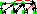
\includegraphics[width=200px]{Images/fig11.pdf} \\

\begin{tabular}{l|l|l|l|l|l|l|l|l}
 vu & V & V & V & V & V & V & V & V
\end{tabular} \\

\begin{tabular}{l|l|l|l|l|l|l|l|l}
 pere & - & 1 & 2 & 3 & 2 & 8 & 8 & 2
\end{tabular} \\

\begin{tabular}{l|l|l|l|l|l|l|l|l}
 d & 1 & 2 & 3 & 4 & 7 & 10 & 12 & 9
\end{tabular} \\

\begin{tabular}{l|l|l|l|l|l|l|l|l}
 f & 16 & 15 & 6 & 5 & 8 & 11 & 13 & 14
\end{tabular} \\

Pile des appels récursifs : \\
u = 7 $\rightarrow$ 6(vu), 8(vu) FINI \\
u = 6 $\rightarrow$ 1(vu), 5(vu) FINI \\
u = 8 $\rightarrow$ $\bar{6}$,$\bar{7}$ FINI \\
u = 5 $\rightarrow$ 1(vu), 4(vu) FINI \\
u = 4 $\rightarrow$ 2(vu) FINI \\
u = 3 $\rightarrow$ $\bar{4}$ FINI \\
u = 2 $\rightarrow$ $\bar{3}$,$\bar{5}$,$\bar{8}$ FINI \\
u = 1 $\rightarrow$ $\bar{2}$,5(vu),8(vu) FINI \\
temps : 16 \\

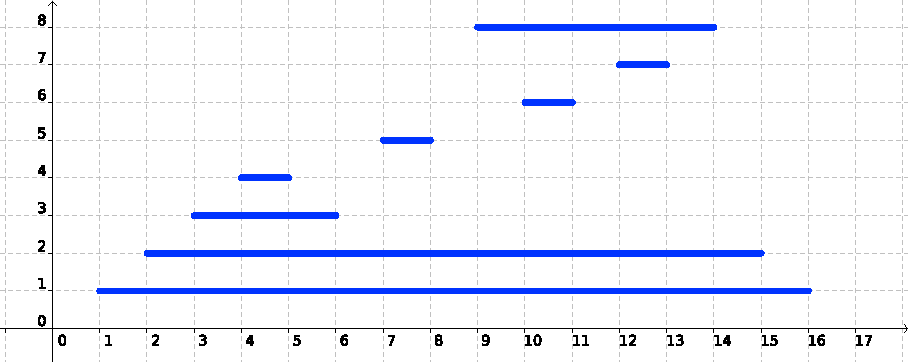
\includegraphics[width=300px]{Images/fig12.pdf} \\
